\documentclass[]{elsarticle}
\usepackage{amssymb,amsmath}
\usepackage{epigraph}

\newcommand{\denote}[1]{\mbox{ $[\![ #1 ]\!]$}}

\usepackage{graphicx,grffile}

\setlength{\parindent}{0pt}
\setlength{\parskip}{6pt plus 2pt minus 1pt}
\setlength{\emergencystretch}{3em}  % prevent overfull lines
\providecommand{\tightlist}{%
  \setlength{\itemsep}{0pt}\setlength{\parskip}{0pt}}
%\setcounter{secnumdepth}{0}

\title{Pragmatic language interpretation as probabilistic inference}

\author[stan]{Noah D. Goodman\corref{cor1}}
% \ead{ngoodman@stanford.edu}
\author[stan]{Michael C. Frank}
% \ead{mcfrank@stanford.edu}

\cortext[cor1]{Corresponding author, please send correspondence to ngoodman@stanford.edu.}
\address[stan]{Department of Psychology, Stanford University, 450 Serra Mall, Stanford, CA 94305}

\begin{document}

\begin{abstract}
Understanding language is more the than use of fixed conventions and more than decoding combinatorial structure. Instead, comprehenders make exquisitely sensitive inferences about what utterances mean given their knowledge of the speaker, the language, and the context.
Building on developments in game theory and probabilistic modeling, we describe the rational speech act (RSA) framework for pragmatic reasoning. RSA models provide a principled way to formalize inferences about meaning in context; they have been used to make successful quantitative predictions about human behavior in a wide variety of different tasks and situations, and they explain why complex phenomena like hyperbole and vagueness occur. More generally, they provide a computational framework for integrating linguistic structure, world knowledge, and context in pragmatic language understanding.
\end{abstract}

\maketitle

\epigraph{... one of my avowed aims is to see talking as a special case or
variety of purposive, indeed rational, behavior ...}{Grice (1975),
p. 47}

\section{Understanding language}
\label{introduction}

Language is central to the successes of our species; with language we
can coordinate our actions, learn from each other, and convey our
innermost thoughts. From sounds to syntax, natural languages provide
structured methods of combining discrete materials to generate an
infinite variety of sentences. Yet this discrete combinatorics does not
fully explain how speakers can use language so flexibly to achieve
social goals. The interpretation of a particular utterance
can itself be almost infinitely variable, depending on factors such as
the identity of the speaker, the physical context of its use, and the
previous discourse. While the systematization of structural features of
language is one of the proudest accomplishments of cognitive science \citep[e.g.,][]{chomsky1965,jackendoff2002,goldberg2003}, its contextual
flexibility -- its pragmatics -- has been stubbornly difficult to
formalize.

\citet{grice1975} presented an initial framework theory for pragmatic
reasoning, positing that speakers are taken to be cooperative, choosing
their utterances to convey particular meanings. Gricean listeners then
attempt to infer the speaker's intended communicative goal, working
backwards from the form of the utterance. This goal inference
framework for communication has been immensely influential \cite[e.g.,][]{horn1984,sperber1986,clark1996,levinson2000}. But
attempts to build on these ideas by providing a specific set of formal
principles that allow the derivation of pragmatic inferences have met
with difficulty.

For example, the core of Grice's proposal was a set of
\textbf{conversational maxims} (see Glossary). Inferences about speakers' behavior relative to these maxims (be truthful,
relevant, informative, and perspicuous) could lead to
\textbf{implicatures} -- inferences about their intended meaning. Formalization of the Gricean notion of
implicature using the maxims is difficult, however, and many
post-Gricean theories have instead proposed alternative sets of
principles \citep{sperber1986,levinson2000}. An important test
of the difficulty of this theoretical project is that the burgeoning
experimental psycholinguistic literature attempting to measure pragmatic
inference has found these principles only modestly useful \citep{breheny2006,huang2009,noveck2008}.
In addition, this sort of informal theory of pragmatics can make only directional,
qualitative predictions with respect to experimental data that are typically graded and
quantitative.

An alternative strand of Gricean thought has had more success in making
contact with data. Grice's core insight was that language use is a form
of rational action; thus, technical tools for reasoning about rational
action should elucidate linguistic phenomena. Such a goal-directed view
of language production has led to the development of engineering systems
for natural language generation \citep{dale1995} that have in turn
been applied as theories of human language production \citep[e.g.,][]{viethen2006}.
Concurrently, the tools of game-theory -- which allow for
the characterization of rational actions with respect to defined
utilities -- have provided a vocabulary for formal descriptions of
pragmatic phenomena \citep[e.g.,][]{benz2006,jager2008}. The recent work we focus on
here builds on these developments, combining them with a more detailed
view of cognition that arises from the Bayesian cognitive modeling
tradition.

Probabilistic, or Bayesian, models have been at the core of a set of
recent attempts to understanding the interplay between structured
representations and graded or statistical information \citep{Tenenbaum2011}.
These models have been an important tool for understanding
non-linguistic varieties of rational action, integrating belief
understanding with action planning \citep{baker2009}. A
critical feature of these models is that they use the probability
calculus to describe inferences under uncertainty. Within formal models
of pragmatics, this uncertainty stems from a variety of sources,
including uncertainty about speakers' goals and beliefs, uncertainty
about the discourse and broader context, and even uncertainty about the
meanings of words.

In the remainder of this paper we describe the probabilistic approach to  pragmatics. We begin by presenting the \textbf{rational speech act
(RSA) model}, and the growing body of empirical data supporting its
utility in explaining pragmatic reasoning. We next discuss extensions
to RSA that allow it to be applied to non-literal uses of language like
hyperbole, irony and metaphor, to cases of vagueness and ambiguity, and
to complex interactions between pragmatics and compositional
syntax/semantics. We close by considering the broader applications of
-- and challenges for -- probabilistic pragmatics models.

\section{A ``rational speech act'' model}\label{a-rational-speech-act-model}

The ``rational speech act'' (RSA) model implements a social
cognition approach to utterance understanding. At its core, it captures
the idea (due to Grice, David Lewis, and others) that speakers are assumed to
produce utterances to be helpful yet parsimonious, relative to some
particular topic or goal. Listeners then understand utterances by
inferring what such a helpful speaker must have meant, given what she
said.\footnote{For clarity throughout, we use a female pronoun for Alice, the speaker, and a male pronoun for Bob, the listener.}
The first of these basic assumptions is formalized by viewing the speaker
as a utility-maximizing agent (where the effort of language production
is costly, but communicating information is beneficial). The listener then
updates his beliefs via Bayesian inference.

The pragmatic listener infers the state of the world, \emph{w,} using
Bayes' rule, given the observation that the speaker chose a particular
utterance, \emph{u}:

$$P_L(w\mid u) \propto P_S(u \mid w)P(w)$$

The key assumption he must make is that the speaker is
\emph{approximately rational,} that is, that she has chosen her
utterances in proportion to the utility she expects to gain.

$$P_S(u\mid w) \propto exp(\alpha
U(u;w))$$

The speaker chooses $u$ from a set of \emph{alternative utterances}
(see Outstanding Questions). The parameter $\alpha$
captures the extent to which the speaker maximizes her utility --
how rational she will be. The basic speaker utility used in RSA
captures the social benefit of providing epistemic help to a listener:

$$U(u;w) = \log P_{\text{Lit}}(w \mid u)$$

This expression measures how certain the listener becomes about the intended world, after hearing the utterance;
in order to avoid an infinite recursion and provide an entry point for conventional (semantic) meaning, the speaker is
assumed to consider a simpler listener, the \emph{literal listener}
$P_{\text{Lit}}$. The literal listener again updates his beliefs in
accord with Bayesian inference, under the assumption that the literal
meaning of the utterance is true:

$$P_{\text{Lit}}(w\mid u) \propto \delta_{\denote{u}(w)}P(w)$$

This definition of the literal listener requires a semantic denotation
for each sentence, $\denote{u}$, in which a sentence
has the value true or false when applied to a particular state of
affairs, $w$ (the ``world'').
This denotation is how conventional meaning enters the pragmatic reasoning process,
and, as we describe briefly below, it connects RSA to work in lexical and
compositional semantics \citep{heim1998,dowty2012}.

%\footnote{Though traditional Montagovian semantics uses binary truth values, it is also in principle possible in this model to use a semantics with real-valued truth functions, and perhaps even to construct a real-valued semantics from vector-based representations \citep{monroe2015}.}

\begin{figure}[t]
\begin{center}
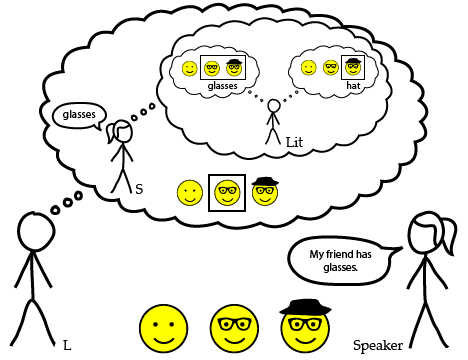
\includegraphics[width=1.0\textwidth]{images/media/image02.png}
\caption{\label{fig:hg} Application of RSA-style reasoning to a signaling
game (shown by the three faces along the bottom). Agents are depicted as reasoning recursively about one another's beliefs: listener L reasons about an internal representation of a speaker S, who in turn is modeled as reasoning about a simplified literal listener, Lit.
Boxes around targets in the reference game denote interpretations available to a particular agent.}
\end{center}
\end{figure}

Consider the scenario in Figure \ref{fig:hg}, in which speaker and listener share a
world of three faces -- one with hat and glasses ({\sc hg}), one with glasses
only ({\sc g}), and one with neither ({\sc n}); one of these (known to the speaker
but not the listener) is the ``friend.'' The speaker says ``my friend
has glasses,'' presupposing that there is a single friend.
Experimental participants, who know that the only alternative utterance was ``my friend has a hat,'' tend to share the intuition that this sentence refers to {\sc g} and not {\sc hg} or {\sc n} \citep{stiller2011,stiller2015}. While real-world language has many more utterances available (e.g., ``my friend has glasses, but no hat''), this restricted scenario serves to illustrate the underlying dynamics of pragmatic reasoning.

Under RSA, listener L reasons about S (a simplified
internal representation of the speaker), who in turn reasons about Lit
(a yet more simplified internal model of the listener). Lit updates his
beliefs based on a straightforward denotation: ``glasses'' applies to
both {\sc g} and {\sc hg}, while ``hat'' applies only to {\sc hg}. Thus
$P_{\text{Lit}}(w\mid \text{``hat''})$ places all probability on the friend
being {\sc hg}, while $P_{\text{Lit}}(w\mid \text{``glasses''})$ places equal probability on {\sc g} and {\sc hg} (see innermost thought bubbles in Figure \ref{fig:hg}). The speaker S who intends to communicate that {\sc hg} is the friend will thus tend to choose the more informative ``hat''; but if she intends to communicate that {\sc g} is the friend, she will use ``glasses.'' Finally, upon hearing ``glasses,'' the listener L infers that this likely refers to {\sc g} (reflecting the counterfactual that if S had been talking about {\sc hg}, she would have said ``hat'' instead).

In the simplest RSA model, as illustrated above, the speaker values
providing epistemic help -- information -- to the listener. But the model can also be extended to create a more sophisticated speaker who is uncertain
about the world state, who avoids costly utterances, or who aims to
provide relevant information. Connections to
other theoretical approaches and aspects of language then become
straightforward. For instance, by modifying the speaker's utility function, we can model the notion of \emph{topic-relevant} information, which
connects to linguistic ideas about the ``question under discussion''
\citep{roberts1996}.
As a second example, RSA can be combined with the noisy
channel approach to language comprehension \citep{levy2008},
in order to explain the communicative use of sentence fragments and prosodic stress \citep{bergen2015}.

In sum, RSA models replace Grice's maxims with a single, utility-theoretic version of the cooperative principle \citep{franke2016b}.
This formulation is based on utilities that can reflect the communicative and social priorities of a complex, real-world agent.

\section{Empirical support for RSA}\label{empirical-support-for-rsa}

The example shown above in Figure \ref{fig:hg} is an instance of a signaling game of the type  initially introduced by \citet{lewis1969}. Such games are a valuable tool for exploring pragmatic inferences in context, and experiments testing the
RSA framework have used games of this type to make quantitative
measurements of a variety of different inferences. For example, one study \citep{frank2012} used a one-shot, web-based paradigm to present
participants with geometric shapes in a variety of different
configurations. Using a betting paradigm (participants were asked to
distribute \$100 between response options), these experiments collected
separate judgments about what a speaker would say, a listener would
interpret, and about baseline expectations for reference (corresponding
to the prior $P(w)$). The RSA model showed a tight fit
to listeners' aggregate judgments when combined
with empirical measurements of the prior distribution:
$P_S$ and $P_L$ models correlated very strongly with participants' average bets on what to say and how to interpret, respectively.

Although in this initial work RSA was used to simulate the behavior of
both speakers and listeners, most subsequent work has focused on the
behavior of listeners alone. This work follows the idea that RSA captures listeners'
(perhaps optimistic) assumptions about the rational behavior of
speakers. Thus, RSA is `rational' in the sense of assuming that
speakers are rational; a separate question is how rational speakers
actually are (\textbf{see Box \ref{proref}}).
In addition, though most research using RSA models has focused on mature language comprehenders, these models have also been the inspiration for a variety of developmental work (\textbf{see Box \ref{box-childrens-developing-pragmatic-competence}}).

A variety of other work has replicated and extended the initial findings
using similar signaling-game paradigms. A tight replication of the
initial results \citep{qing2015} reproduced the basic findings and
explored a set of variants to the initial RSA utility function.
Other studies \citep{carstensen2014} found that RSA
predicted judgments in a communication game using much more complex
spatial language stimuli, albeit with somewhat noisier fits. Thus, RSA
with an epistemic utility can predict judgments in simple signaling
games across variations in both participant sample and stimulus.

One question raised by this initial work was the level of {\bf social recursion} (see Glossary) that
best fit human performance. The presentation of RSA given above is
stated in terms of a minimal recursion (a listener reasons about
speaker, who in turn reasons about a literal listener) but much greater
depths of reasoning are in principle possible. The evidence is mixed on whether deeper levels of recursion are commonly seen in language comprehension. In a variety of experiments exploring this issue, participants tended to show chance-level performance for signaling systems that required deeper levels of
recursion to find unique interpretations \citep{stiller2011,degen2012,vogel2013}. More recent studies \citep{franke2016},
however, showed some evidence of deeper recursion
for a subpopulation of participants (approx.~15\%) in a more
complex paradigm, consistent with work on competitive economic
games where deeper recursions are sometimes found \citep{camerer2004}. This heterogeneity -- and its dependence
on individual and contextual differences -- is an interesting topic for
future work.

A number of other studies have tested RSA with more elaborated utility functions (\textbf{see Box on Refinements to the speaker’s utility}). For instance, a speaker might be expected to
produce a less informative utterance when the more informative one is
much harder to say. This tendency can be formalized by including a cost
term in the speaker's utility; with this modification, RSA
predicts the impact of production costs on interpretations of the
listener. Work exploring this extension \citep{bergen2012} showed that participants in a reference
game are indeed sensitive to the cost of
message choices: the effect of alternative possible messages on a listener's inferences is modulated by their cost, in dollars. Related studies \citep{degen2013} tested the effect of production
difficulty by manipulating how quickly the speaker could type on an
on-screen keyboard; participants' interpretations reflected this difficulty
as predicted. Additional work has used proxies for production cost
such as number of words and their frequencies in explorations of phenomena such as negation \citep{nordmeyer2014} and the choice of noun used to refer to an object \citep{graf2016}.

Finally, in addition to ad-hoc signaling systems, RSA provides a way to describe reasoning about classic linguistic
implicatures. Perhaps the
best-studied of these is the scalar implicature that ``some of the
letters had checks inside'' implicates that not all did.
One study \citep{goodman2013} measured participants' judgments about the
interpretations of quantifiers and number words in exactly this
situation and found that these judgments were well-predicted by RSA. In
addition, a critical feature of this study was the inclusion of an
epistemic manipulation (e.g., whether all of the letters had already been opened). By using expected informativity (\textbf{see Box}) to account for the speaker's
limited perceptual access, the model was able to predict
differing patterns of listener judgments based on different levels of
speaker uncertainty. These empirical findings are congruent with other recent
demonstrations of the importance of epistemic reasoning in pragmatic
implicature \citep{bergen2012,breheny2013}, and the theoretical account accords with other probabilistic treatments of scalar implicature \cite{russell2012}. They
also highlight the way the RSA framework provides a (non-modular) theory
for interactions between language and non-linguistic cognition.
We next turn to a variety of other extensions to the basic RSA model that explore additional interactions.

\section{Uncertainty about the speaker: Joint reasoning}\label{uncertainty-about-the-speaker-joint-reasoning}

In the basic RSA model, the listener has a specific model in mind of how
a speaker will behave. But what should a listener do if he is not sure
what speaker model is appropriate? Speakers can differ in knowledge, communicative goals, and many other aspects;
these differences can lead a listener to arrive at different interpretations of the same utterance.
Recent work has addressed this issue by positing a joint inference: What type of speaker am I
interacting with and what is the world like, given the utterance I
heard? Formally this \emph{uncertain} RSA (or uRSA) framework requires
only a small change:

$$P_L(w,s\mid u) \propto
P_S(u\mid w,s)P(s)P(w)$$

where the new variable $s$ parametrizes different speaker types. In practice, $s$ can
refer to any factor that might influence the speaker's behavior,
including uncertainty about conversational topic, word
meanings, background knowledge, or general discourse context.
This modification allows uRSA to capture a much wider variety of
linguistic phenomena; intuitively, an uRSA listener is a more realistic
cognitive agent than the RSA listener, who was restricted to the
specifics of a very particular context and goal. To illustrate this
intuition, we provide three examples of phenomena captured by uRSA (but not by basic RSA): non-literal language, vagueness, and embedded implicatures.

Non-literal or figurative language -- utterances that are easily interpreted but not
``actually true'' -- poses a problem for nearly all formal models of language
understanding. How can tropes like
hyperbole, sarcasm, and metaphor be interpreted, and why are they used?
Under uRSA, these uses can be described as arising from uncertainty
about the topic of conversation. If the speaker is expected to provide
information relevant for a particular topic,
the pragmatic listener will only update his beliefs along this topical
dimension. Within uRSA, the interaction between uncertainty about the speaker's
intended topic and her intended meaning about that topic can drive
complex interpretations.

\begin{figure}[ht]
\begin{center}
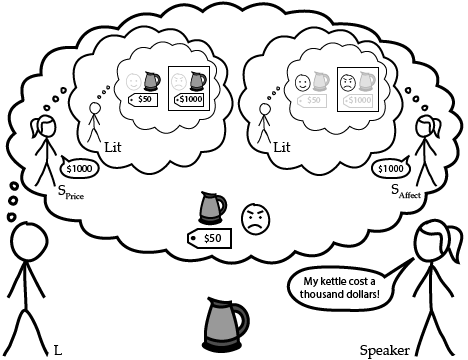
\includegraphics[width=1.0\textwidth]{images/media/image03.png}
\caption{\label{fig:ursa} Uncertain RSA-style reasoning applied to hyperbole. Listener L reasons jointly about the price of the item and the speaker's affect. In doing so he considers two speakers, one who is primarily interested in conveying her affective response to the kettle, and one who is primarily interested in conveying the actual price. (The full model also considers speakers, not pictured, that wish to convey approximate price and combinations of these goals.) Each of these speakers is modeled as reasoning about a literal listener who interprets the utterance literally (indicated by the box selecting the ``\$1000'' state), but focus on different aspects of the situation (price on the left and affect on the right).}
\end{center}
\end{figure}

Hyperbolic utterances such as ``the
electric kettle cost \$1,000'' are a key case study \citep{kao2014}.
In this example, the number \$1,000 can be
interpreted as conveying information about the speaker's affect, not the
actual price, in part because one thousand dollars is an implausibly
high price for a kettle. As shown in Figure \ref{fig:ursa}, the uRSA model  captures this intuition by positing that the topic of the speaker's
utterance may be the actual price of the kettle, the speaker's
opinion about the price, or some combination of the two. Since the listener
does not know the topic, he jointly infers it together with the
likely true price of the kettle and the speaker's affect. When the
uttered price is implausible it becomes more likely that the speaker is aiming to convey her opinion,
and using \$1,000 (a price which most people would find too high) to do so.
In this way, the listener's joint inference can yield a
non-standard topic and hence a non-literal interpretation.

By extending
the space of affect to include both valence and arousal, the same model predicts verbal irony \citep{kao2015}.
And a similar approach has been suggested for simple
metaphors \citep{kao2014b}, such as ``John is a shark.''
Here the potential topics include not affect, but features of the
target, such as how vicious John is and how likely he is to swim
underwater. In each of these cases of figurative language, the uRSA model accounts for almost all of the explainable variance in
human interpretations, a striking result considering the complexity and subtlety of these phenomena.

Many linguistic descriptions, especially adjectives, are both context-sensitive and vague. Providing precise definitions for words like \emph{expensive} or \emph{tall} has been a persistent challenge for philosophers and semanticists \citep{williamson2002}. uRSA models address this challenge by assuming that word meanings can differ between speakers and contexts, and and that these meanings themselves can be a subject for inference. In the case of scalar adjectives like \emph{tall}, the uncertainty is over the threshold required: what height is required before an object counts as tall?
Under the uRSA model, judgments about meaning take into account two conflicting pressures: On one hand, a stricter threshold for tallness makes the term \emph{tall} more informative. For instance ``Bob is tall'' tells us a great deal if \emph{tall} requires a height greater than eight feet. But, on the other hand, a stricter threshold makes such a sentence quite unlikely to be true \emph{a priori}.
By negotiating this balance between informativity and plausibility, uRSA accounts for three key phenomena of vague adjectives \citep{lassiter2015}: the inferred meaning depends on the class (tall for a tree vs. tall for a person), there are borderline cases, and the interpretations are subject to a \emph{sorites} paradox (no single minimal increment in height will make you tall, but enough increments will). The process of reasoning about meaning that are modeled by uRSA might even interact with learning processes to produce more long-lasting inferences about word meaning, leading to language change (\textbf{see Box on Language use and language change}).

% This approach to uncertainty about word meanings has been extended to account for effects generic and habitual
% statements \citep{tessler2016} and manner implicatures \citep{bergen2016}.


% For instance, scalar adjectives like \emph{tall} and \emph{expensive} have an extremely
% flexible meaning -- a \emph{tall man} is quite different in height than
% a \emph{tall building}. In these cases, uRSA models can be used to infer
% the precise meaning of words \citep{bergen2016}.

Finally, this uRSA approach allows for progress on an important puzzle
in recent discussions of pragmatic inference: embedded implicature \citep{geurts2009,chemla2011}. Embedded
implicatures occur when quantifiers are nested within one another, as in
sentences like ``Exactly one letter is connected with some of its
circles.'' In these cases, some experimental evidence suggests that
participants access the interpretation that one letter is connected with
some \emph{but not all} of its circles, an interpretation that standard
Gricean theories cannot generate \citep{chemla2011}.
Recent work \citep{potts2015} has replicated these interpretations in a series of large-scale
experiments and confirmed that basic RSA models could not capture them.
An implementation of uRSA that jointly infers word meanings and world state \citep{bergen2016,potts2015} showed a good fit to the overall pattern of data. Sentence meanings in this model are built by composing uncertain word meanings, showing how uRSA is a fruitful way to incorporate pragmatic reasoning into compositional semantic systems.

\section{Concluding remarks and future directions}\label{conclusions-and-future-directions}

Context-dependence is one of the core features of natural language. Yet
because of the informal nature of theorizing about this context-dependence,
pragmatics has often been treated as a theoretical ``wastebasket,'' in
which unexplained phenomena are hidden \citep{bar-hillel1971}. Countering this trend, new formal theories of pragmatics make quantitative
predictions about a wide variety of phenomena that have previously been
considered too difficult to operationalize. These include implicature,
vagueness, non-literal language, and the myriad other cases where
linguistic meaning is changed by context.

The key tool in this work is the Rational Speech Act framework, which builds upon and synthesizes a
number of formal traditions in the study of human inference, from game
theory to models of human reasoning.
The RSA approach also builds on existing
work on semantic representation -- using a compositional semantics
\emph{a la} Montague \citep{dowty2012} -- and contributes back to semantics, providing a
specific mechanism by which underspecified meanings become precise, in
context.
Rather than formalizing only a single hypothesis about pragmatic language understanding,
RSA provides a framework in which many variations can be explored.
Varying assumptions about the speaker's utility (\textbf{see Box: Refinements to the speaker's utility})
and listener's uncertainty (see Section \ref{uncertainty-about-the-speaker-joint-reasoning}), for instance,
yields a spectrum of hypotheses that can be evaluated against quantitative experimental data.

While it has been successful in many recent cases, it may emerge that the RSA approach is not able to capture
some aspects of language understanding, either because the foundational, Bayesian, tools it relies on are inadequate \citep{jones2011}, or because pragmatic effects arise from sources not easily incorporated into RSA.
Optimistically, however, RSA can be combined with other approaches when needed.
For instance, the alternative utterances in RSA can be restricted  \citep{potts2015} using previously-proposed grammatical mechanisms \citep{Fox2011}. And increasingly, methods in machine learning have been used to supplement RSA with powerful learning mechanisms \cite{monroe2015}.
Indeed, this cross-fertilization is among the most encouraging outcomes of work on RSA.




% Future work will need to engage with additional levels of linguistic structure, such as discourse (Ascher, etc).

The RSA framework is a \emph{computational} level description of the
language user's competence, in Marr's sense \citep{marr1982}.
There are many
possible ways a cognitive agent could implement RSA at the algorithmic
level, and it is unclear which might match the speed and competence of human language understanding and production.
These alternatives must further be evaluated for their ability to explain the processing signatures of language comprehension such as reaction times and eye gaze \citep{degen2015,nordmeyer2014}.
Yet even as a computational-level framework, RSA inspires different intuitions about processing than previous theories.
For example, RSA-style reasoning makes pragmatic inferences a fundamental part of language comprehension,
in which the ultimate goal of all interpretation is to settle on the intended
meaning, given both the literal semantics of the utterance and the
broader pragmatic context.
This framing contrasts with Gricean analyses, in which pragmatics enters when the violation of a maxim leads to reasoning
to ``repair'' the interpretation, and correspondingly slower processing, a view that has been
challenged both theoretically and empirically \citep[e.g.,][]{levinson2000,grodner2010}.

%Yet even in its
%current form, RSA potentially suggests a new take on pragmatic language
%processing -- one that is consistent with recent empirical
%findings.
%In Gricean analyses, a violation of a maxim leads to reasoning
%to ``repair'' the interpretation. Many theorists have inferred from this
%idea of repair that pragmatic inferences should be slow (because they
%depend on full semantic interpretation) and optional (because they only
%happen after a violation). These assumptions have been
%challenged both theoretically and empirically \citep[e.g.,][]{levinson2000,grodner2010}.
%In this way, RSA is consistent with modern
%psycholinguistic theories that emphasize interactive, incremental
%processing \citep{degen2015}.



Future extensions of RSA will likely include worlds with more and richer structure;
a thorough and practical theory of pragmatic alternatives;
more sophisticated discourses that unfold over many utterances;
and utility structures that better take into account the complexities of social interaction.
On the practical side, computing the predictions of RSA models can
become prohibitive when the number of world states or utterances grows
large. Further development of algorithms to implement RSA is needed.
These
developments may go together with new algorithms for learning aspects of
the underlying semantics, which will open up new applications for the
RSA approach in computational linguistics and artificial intelligence \citep{golland2010,vogel2013b,monroe2015,andreas2016, orita2014}.
% (e.g., Goland, Liang, \& Klein, 2010; Vogel \& Potts, 2013; Munroe \&
% Potts, 2015; Andreas \& Klein ??).

The work outlined in this review represents steps towards a
comprehensive, formal theory of language understanding in context. Although
much further work will be required, RSA models and their uRSA extensions have
proven to be useful tools for explaining both qualitative and
quantitative empirical data across a wide range of tasks and contexts.
Language is central to the human experience. We hope our work sheds
light on how its structure and systematicity can still give rise to such
an astonishingly flexible communication system.

\section{Acknowledgements}

We gratefully acknowledge funding from a James S. McDonnell Foundation Scholar Award to Goodman,
 ONR Grants N00014-13-1-0788 and N00014-13-1-0287 to Goodman and Frank, and NSF BCS Grant 1456077 to Frank.

%\appendix


% --------------------------- OTHER MATERIALS ------------------------


\section{Trends}\label{trends-box}

\begin{itemize}
\item Rational speech act (RSA) models provide a quantitative framework to
  capture intuitions about pragmatic reasoning in language
  understanding.
\item Extensions to RSA that allow for reasoning about the speaker -- for instance, her goals and word usage -- can capture many otherwise puzzling phenomena
  including vagueness, embedded implicatures, hyperbole, irony, and
  metaphor.
\item The RSA framework can inform psycholinguistic processing experiments,
  linguistic theory, and scalable natural language processing models.
\end{itemize}

\section{Box: Outstanding questions}\label{box-outstanding-questions}

\begin{itemize}
\item \emph{Social recursion.} How deeply do human comprehenders reason about others' intentions? Is depth of recursion -- ``I think that you think that...'' -- constant, or does it vary across situations?

\item \emph{Alternatives.} How are alternative utterances computed? Do they depend on the language grammar? On situational factors?
  %  Do they depend \emph{a priori} on the heard utterance ofcontext?

% \item \emph{Learning}. How can pragmatic reasoning occur in situations where
%   an agent has uncertainty about the meanings of words or how they are
%   combined?
%
\item \emph{Linguistic goals}. How do ``Gricean'' utilities -- the drive to be informative yet succinct -- relate to other social goals like conveying affect, or establishing relationships? How do cooperative and competitive goals mix in language use?

\item \emph{Dialogue}. How can RSA be used to model the evolution over the course of a conversation of a partners' utilities, possible goals, and the context more broadly?

 \item \emph{Learning and language change}. How do pragmatic language understanding and language learning interact? How and when does pragmatic language use lead to language change?

\item \emph{Algorithmic challenges}. Given the potential complexity of
recursive pragmatic computations, how is language processed so quickly? How can RSA models be ``scaled up'' for natural language
  processing tasks?
%
% \item \emph{Neural mechanisms.} What are the neural substrates of pragmatic
%   language comprehension, and are they shared with other mentalistic reasoning?

\end{itemize}

\section{Box: Refinements to the speaker's utility}\label{box-refinements-to-the-speakers-utility}

The notion of the speaker's utility -- what is rewarding for a speaker -- is central to the RSA approach. The basic RSA model captures the speaker's need to be \emph{informative} to a listener: $U(u; w) = \log P_{\text{Lit}}(w\mid u)$. Different utilities lead to different kinds of
speakers, which in turn lead to different interpretations by the pragmatic
listener. Several utility refinements (and their combinations) have been
considered in recent work:

\begin{itemize}
\item Utterance cost: In order to capture a tendency of speakers to be
  parsimonious we can simply add a cost term: $U(u; w) =
  \log P_{\text{Lit}}(w\mid u) + cost(u)$. The cost may
  reflect actual production cost (such as number of words) or proxies
  such as word frequency. This extension yields effects similar to
  Grice's maxim of manner \citep{bergen2016}.

\item Speaker uncertainty: When the speaker does not have full knowledge of
  the world she should choose an utterance according to \emph{expected
  utility}: $U(u;k) = {\mathbb E}_{P(w\mid k)}{[}U(u;w){]}$, where $k$
  summarizes the speaker's knowledge or observations. This extension
  correctly predicts interactions between a speaker's knowledge and a
  listener's interpretations \citep{goodman2013}.

\item Topic relevance: Although it may be highly informative to provide detailed descriptions, such detail is not always relevant. Relevance can be captured by introducing a topic of conversation \citep[sometimes known as a \emph{Question Under Discussion,}][]{roberts1996} and adjusting the epistemic utility to reflect only information about this topic: $U(u;w,t)=\log \sum_{w' \text{ s.t. } t(w')=t(w)} P_{\text{Lit}}(w'\mid u)$. Here the topic is encoded in a function $t$ that takes a complete world and yields some subset or summary; for instance, in the case of hyperbole \citep{kao2014}, $t$ can pick out only the speaker's affect, dropping objective states.
%Because the topic may reflect previous interactions, this extension leads to a variety of discourse effects.

\item Other social goals: Language is often used not just to inform, but
  also to flirt, insult, comfort, and to pursue myriad other social
  goals. For example, non-informational utilities, e.g. utility directed towards
  kindness, can produce behaviors that appear polite \citep{yoon2016}.

\end{itemize}

\section{Box: RSA and children's developing pragmatic competence}\label{box-childrens-developing-pragmatic-competence}

From a very early age, children are oriented towards communication, understanding the function of language for information
transfer and repurposing their limited linguistic means to achieve a
wide variety of ends \citep{vouloumanos2012,clark2010}. In light
of this general early orientation, the literature on pragmatic
development specifically has been puzzling: older children very reliably
fail to make scalar implicatures under a range of circumstances \citep{noveck2001}. In one striking example, five-year-olds endorsed the statement that ``some of the horses jumped over the fence'' even when three out of three of a set of horses had made the jump \citep{papafragou2003}. RSA-style models can provide a framework for thinking about this disconnect between early communicative successes and
later pragmatic failures.

Recently, theorists have proposed that children's apparent difficulties with
pragmatic implicatures may have resulted from their inadequate
knowledge of relationships between lexical alternatives rather than
difficulty with pragmatic computations more generally \citep{barner2011}. Congruent with this idea, three-year-old children show
signs of successful implicature computations in the kinds of signaling games shown in Figure \ref{fig:hg}, where the referential alternatives are all simple objects that are visible in the scene \citep{stiller2015}. And children in the same age range were able to use an
implicature to guess the meaning of a novel word \citep{frank2014} or a novel context \citep{horowitz2016}, showing the kind of inferential flexibility posited in RSA accounts.

These findings support the idea that even young children are able
to make flexible pragmatic inferences, and are consistent with the application of RSA-style reasoning, albeit with limits on the available semantic alternatives. Future
research will be required, however, to test whether RSA (or some
capacity-limited modification) could make quantitative predictions about
pragmatic development.

\section{Box: Producing referring expressions}\label{box-producing-referring-expressions}
\label{proref}

RSA stands for the ``rational speech act'' model, indicating that listeners idealize speakers as rational.
Are speakers in fact rational in a meaningful way? And if so, how can this conclusion be
integrated with the large body of evidence indicating that speakers are
egocentric, error prone, and subject to idiosyncratic production
preferences \citep{keysar2003,lane2006,gatt2013}?
% (Keysar et al., 2003; Lane, Groisman, \& Ferreira, 2008; Gatt et al., 2013)?

Although our initial studies collected judgments about language
production in extremely restricted tasks \citep{frank2012}, most
recent work using the RSA model has focused on modeling listeners'
judgments, rather than speakers' productions. One reason for this
choice is that often the most interesting pragmatic inferences come
about when speakers are not maximally informative. For example, in the
signaling game shown in Figure \ref{fig:hg}, helpful speakers will often
overspecify and say ``glasses and no hat'' \citep{baumann2014}.
But this unnecessarily redundant utterance may in fact be a
reasonable response to uncertainty about whether a conversational
partner will in fact draw the desired implicature.
%
More generally, speakers' production choices are a promising area for
future research using RSA models with a broader range of utility
functions (see Box) and various sources of potential miscommunication (a topic of ongoing research).

% In the example above, the pragmatic speaker's
%utility would take into account both the costs of production (adding
%``and no hat'') and the likely costs of errors in comprehension by the
%listener (the ``huh? which one?'' that might occur if the listener fails
%to make the implicature -- or simply wants to be absolutely certain).
%Intuitively, this tradeoff might lead to some of the observed patterns
%of ``irrational'' behaviors: for example, if a speaker is less certain
%of the denotation of a gradable adjective like ``big'' then she might be
%more likely to use a color term as well \citep{gatt2013}.

Nevertheless, it is clear that in their natural behavior, speakers make
production decisions under time pressure and a variety of cognitive
demands \citep{levelt1993}. Integrating these demands with the predictions of
utility-theoretic models should be an important challenge for future
work.

\section{Box: Language use and language
change}\label{box-language-use-and-language-change}

The pragmatic processes described by RSA models occur in the moment of
communication, but can have a set of effects that ripple out through
language as a whole. The construal of an individual communication event
can influence learning processes, which in turn can lead to
systematic changes in word meanings \citep{smith2013}.
Words that are too narrow in their denotation can be pragmatically
extended \citep{kao2014}, while words that are too
broad can be narrowed via implicature. Over time, word meanings may
converge to the appropriate level of ambiguity to enable efficient
communication \citep{piantadosi2012}.
In this sense, in-the-moment pragmatic interpretation may bootstrap long term language change.

The processes of change that promote efficient communication have been
explored extensively within the iterated learning paradigm \citep{kirby2008}.
%For example, iterated transmission of an arbitrary communication system can lead to the emergence of semantic regularities \citep{kirby2008}.
This framework can also be used to express the competing pressures of
learnability and communication. When languages are selected only to be
learnable, they often become degenerate, including only a single word
\citep{perfors2014}. But when they include a countervailing
pragmatic pressure, which can be modeled via RSA, expressive and compositional languages can emerge
\citep{kirby2015}.

If pressures for efficient communication lead to language change, then
these pressures should be visible in the lexicons of human languages. Indeed, a
recent body of evidence suggests that the typological distribution of languages in particular
semantic domains reflects the range of optimal communication systems
\citep[e.g.,][]{regier2007,kemp2012,xu2014}.
An important future direction is to understand whether this typological distribution is predicted to arise from iterated learning with a population of RSA-like language users.

%For example, although an infinity of possible ways of
%expressing kinship relations are in principle possible, those that are
%instantiated in natural languages tend to be a good balance between
%expressivity and compression. And some recent evidence suggests that
%communicative regularities may even be encoded at the level of the
%entire lexicon \citep{lewis2016}.

\section{Glossary}\label{glossary}

\begin{itemize}
\item \textbf{Rational speech act model (RSA)}. A class of probabilistic model that assumes that language comprehension in context arises via a process of recursive reasoning about what speakers would have said, given a set of communicative goals.

\item \textbf{Uncertain RSA models (uRSA)}. A specific extension of RSA models that allow for joint inferences about both the speaker's intended meaning and other aspects of the interaction, such as the topic, the context, or even the meanings of particular words.

\item \textbf{Implicature}. An inference about the meaning of an utterance in context that goes beyond its literal semantics. Implicatures are typically \emph{cancellable} in that they can be contradicted, as in ``Some of the students passed the exam; indeed, all of them did.''

\item \textbf{Scalar implicature}. An implicature that arises when a speaker didn't use a stronger alternative term, leading to narrowing of the interpretation. For instance, hearing ``some'' usually leads to a scalar implicature that ``not all.''

\item \textbf{Conversational maxims}. A set of principles described by \citet{grice1975} as a theory of how listeners reason about speakers' intended meaning to arrive at pragmatic implicatures.

\item \textbf{Social recursion}. Reasoning that involves two people, such as listener and speaker, thinking about each other: ``I think that you think that I think that....'' This may proceed to a finite depth, or continue \emph{ad infinitum}.

%Some more that Becca sugested:
%literal listener
%compositional semantic systems
\end{itemize}


\bibliographystyle{model5-names}
%\biboptions{authoryear}
\bibliography{pragmaTICS.bib}



\end{document}
